%\documentclass{beamer}
\documentclass[aspectratio=169]{beamer}
\usetheme{Boadilla}
%\usetheme{Warsaw}
%\setbeamercovered{transparent}
\beamertemplatetransparentcoveredhigh
\usepackage[portuges]{babel}
\usepackage[utf8]{inputenc}
\usepackage{lmodern}
\usepackage[T1]{fontenc}
\usepackage{hyperref} 
\usepackage{listings}
\usepackage{color}

\definecolor{dkgreen}{rgb}{0,0.6,0}
\definecolor{gray}{rgb}{0.5,0.5,0.5}
\definecolor{mauve}{rgb}{0.58,0,0.82}

\lstset{frame=tb,
  language=C,
  aboveskip=3mm,
  belowskip=3mm,
  showstringspaces=false,
  columns=flexible,
  basicstyle={\small\ttfamily},
  numbers=none,
  numberstyle=\tiny\color{gray},
  keywordstyle=\color{blue},
  commentstyle=\color{dkgreen},
  stringstyle=\color{mauve},
  breaklines=true,
  breakatwhitespace=true,
  tabsize=3
}
\title[Ordenação por Seleção]{Ordenação por Seleção\\
   Algoritmos e Estrutura de Dados I}
\author[IEng - UFMT]{Instituto de Engenharia -- UFMT}
%\institute[2020/2]{Segundo Semestre de 2020}
\date{}


\begin{document}

%------------------------------------------------
\begin{frame}[plain]
  \titlepage
\end{frame}

%------------------------------------------------

\begin{frame}
\frametitle{Roteiro} % Table of contents slide, comment this block out to remove it
\tableofcontents % Throughout your presentation, if you choose to use \section{} and \subsection{} commands, these will automatically be printed on this slide as an overview of your presentation
\end{frame}

%----------------------------------------------------------------------------------------
%	PRESENTATION SLIDES
%----------------------------------------------------------------------------------------

%------------------------------------------------
\section{Objetivos}

\begin{frame}
\frametitle{Objetivos}
Esta aula tem como objetivos:

\begin{enumerate}
\item Apresentar os conceitos básicos sobre ordenação;
\item Explicitar os métodos de ordenação SelectionSort e InsertionSort;
\item Exemplificar a execução dos algoritmos.
\end{enumerate}
\end{frame}


%------------------------------------------------
\section{Introdução} % Sections can be created in order to organize your presentation into discrete blocks, all sections and subsections are automatically printed in the table of contents as an overview of the talk
%------------------------------------------------

\begin{frame}
\frametitle{Introdução}
\begin{block}{Ordenar}
 Ordenar é o processo de rearranjar um conjunto de objetos em uma ordem ascendente ou descendente.
\end{block}
\begin{itemize}
\item A ordenação visa facilitar a recuperação posterior de itens do conjunto ordenado;
\item As técnicas de ordenação permitem apresentar um amplo de algoritmos distintos para resolver uma mesma tarefa.
\end{itemize}
\end{frame}

\begin{frame}
\frametitle{Introdução}
 Existem três razões práticas para estudar os algoritmos de ordenação:
\begin{itemize}
\item Analisar os algoritmos de ordenação é uma introdução completa as técnicas de comparação de desempenho de algoritmos;
\item Técnicas semelhantes são eficazes no tratamento de outros problemas;
\item Muitas vezes usamos algoritmos de ordenação como ponto de partida para resolver outros problemas.
\end{itemize}


Mais importante do que esses motivos práticos é que os algoritmos são elegantes, clássicos, e eficazes.
\end{frame}

%------------------------------------------------

\begin{frame}
\frametitle{Notação}
\begin{itemize}
\item Em geral, os elementos do vetor a ser ordenado são objetos complexos, com muitos campos.
\item Do ponto de vista da ordenação, apenas um desses campos -- a chave (= key) -- é relevante. 
\item Vamos supor, para simplificar, que a chave é o único campo do objeto. 
\end{itemize}
\end{frame}

%------------------------------------------------

\begin{frame}
\frametitle{Características}
\begin{itemize}
 \item Qualquer tipo de chave, sobre o qual exista uma regra de ordenação bem definida, pode ser utilizada;
    \begin{itemize}
     \item As ordens mais usadas são a numérica e a lexicográfica.
    \end{itemize}
\end{itemize}    
\begin{figure}[!h]
  \centering
  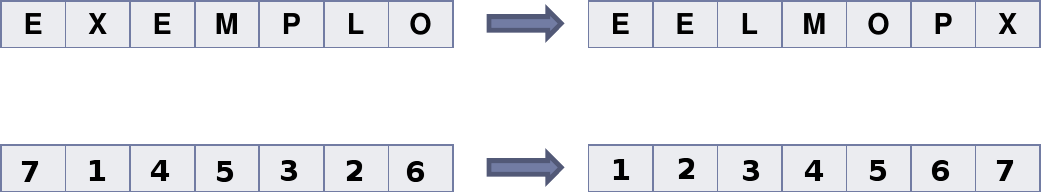
\includegraphics[width=300pt]{imgs/numerica_lexicografica.png}
  \label{fig_numerica_lexicografica}
\end{figure}
\end{frame}

%------------------------------------------------
\section{SelectionSort}
%------------------------------------------------

\begin{frame}
\frametitle{SelectionSort}
\begin{itemize}
 \item Um dos algoritmos de ordenação mais simples; 
 \item A cada iteração, seleciona o menor elemento da lista e troque-o com o item na posição correta;
% \item É realiza uma troca a cada iteração.
 \item Passos para o algoritmo, dado um vetor v[1..n]:
    \begin{itemize}
    \item Procurar o menor elemento no vetor v[1..n] e trocar com o elemento na 1ª posição.
    \item Procurar o menor elemento no vetor v[2..n] e trocar com o elemento na 2ª posição.
    \item Proceder assim até a ordenação estar completa.
    \end{itemize}
 \end{itemize}
\end{frame}

\begin{frame}
\frametitle{SelectionSort}
\begin{figure}[!h]
  \centering
  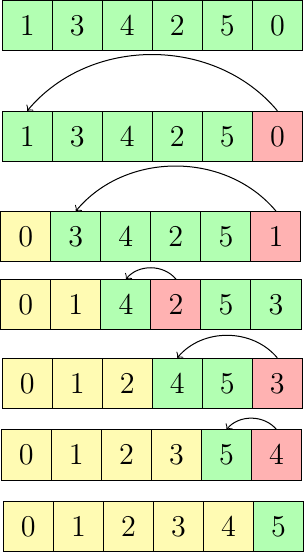
\includegraphics[width=100pt]{imgs/selectionsort.png}
  \label{fig_selectionsort}
\end{figure}
\end{frame}

%------------------------------------------------

\begin{frame}[fragile]
\frametitle{Pseudo-código SelectionSort}
\begin{lstlisting}
void selectionsort(int V[], int n) {
  int i, j, min, aux;  
  for (i = 0; i < n-1; i++) {
    min = i;
    for (j = i+1; j < n; j++) {
      if (V[j] < V[min]) {
        min = j;
      }
    }
    aux = V[i];
    V[i] = V[min];
    V[min] = aux;
  }
}
\end{lstlisting}

\end{frame}


%------------------------------------------------

\begin{frame}
\frametitle{Análise SelectionSort}
\begin{itemize}
 \item Ciclo interno apenas faz comparações
 \begin{itemize}
    \item troca de elementos é feita fora do ciclo interno;
    \item cada troca como um elemento na sua posição final;
    \item o número de trocas é $n-1$ (por que não $n$?).
    \item o tempo de execução é dominado pelo número de comparações.
 \end{itemize}
\end{itemize}

\end{frame}

%------------------------------------------------

\begin{frame}
\frametitle{Características}
\begin{block}{Vantagens}
  \begin{itemize}
  \item Custo linear no tamanho da entrada para o número de movimentos de registros;
  \item É o algoritmo a ser utilizado para arquivos com registros muito grandes (que possuem alto custo de movimentação);
  \item É muito interessante para arquivos pequenos.
  \end{itemize}
\end{block}
\begin{block}{Desvantagens}
  \begin{itemize}
  \item O fato do arquivo já estar ordenado não ajuda em nada, pois o custo continua quadrático;
  \end{itemize} 
\end{block}
\end{frame}

%------------------------------------------------

\begin{frame}
\frametitle{Conclusão}
\begin{block}{Ordenação}
  \begin{itemize}
   \item A tarefa de ordenação é muito importante, ela é uma necessidade básica para a solução de muitos problemas.
   \item Material para reforçare a aprendizagem:
      \begin{itemize}
       \item \href{https://www.youtube.com/watch?v=zjcGGqskf5s}{Vídeo-aula selection sort}
      \end{itemize}

  \end{itemize}  
\end{block}
\end{frame}

%------------------------------------------------

\begin{frame}
\Huge{\centerline{Dúvidas}}

\begin{figure}[!h]
  \centering
  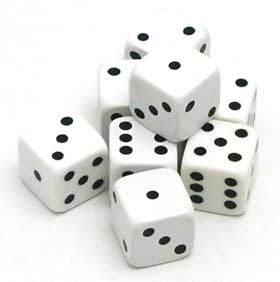
\includegraphics[width=100pt]{imgs/dados.jpg}
  \label{fig_fim}
\end{figure}

\end{frame}

%----------------------------------------------------------------------------------------


\begin{frame}
  \frametitle{Fim}
\begin{center}
\Huge Fim
\end{center}
\end{frame}


\end{document} 